An op amp having a low-frequency gain of $10^{3}$ and a single-pole rolloff at $10^{4}$ rad/s is connected in a negative feedback loop via a feedback network having a transmission k and a two-pole rolloff at $10^{4}$ rad/s. Find the value of k above which the closed-loop amplifier becomes unstable.
\begin{enumerate}[label=\arabic*.,ref=\theenumi]

%\begin{enumerate}[label=\thesection.\arabic*.,ref=\thesection.\theenumi]
\numberwithin{equation}{enumi}
\renewcommand{\thefigure}{\theenumi.\arabic{figure}}

\item Find Open Loop Gain, $G(s)$\\
\solution Gain for an amplifier whose transfer function is characterised with a single pole is-
\begin{align}
    G(s) &= \frac{G_{o}}{1+ \frac{s}{w_{p}}}
\end{align}
Here, $G_{o}$ is low frequency gain and $w_{p}$ is pole frequency. Thus for our problem,
\begin{align}
\label{eq:olg}
    G(s) &= \frac{10^3}{1+\frac{s}{10^4}}
\end{align}

\item Find Feedback factor, $H(s)$\\
\solution Given transmission(=low freq. gain) and two pole roll-off at $10^4$rad/s.
\begin{align}
    H(s)&= \frac{k}{\left(1+\frac{s}{10^4}\right)^2}
\end{align}

\item Loop Gain, G(s)H(s)\\
\solution 
\begin{align}
    G(s)H(s) &= \frac{10^3k}{\left(1+\frac{s}{10^4}\right)^3}
\end{align}

\item Stability of the Closed Loop Amplifier\\
\solution Closed loop systems stability can be tested by examining the Gain Margin, or Phase Margin alternatively. First, let's find $\omega_{180}$, the phase cross-over frequency
\begin{align}
       \angle G(j\omega)H(j\omega) =  \angle\frac{10^3k}{\left(1+\frac{j\omega}{10^4}\right)^3}\\
       \implies -3tan^{-1}\left({\frac{\omega}{10^4}}\right)
\end{align}
At $\omega = \omega_{180}$,
\begin{align}
       -180^{\circ}= {-3tan^{-1}\left({\frac{\omega_{180}}{10^4}}\right)}\\
        \implies \omega_{180} = \sqrt{3}\times 10^4
\end{align}
For a stable system, $GM_{dB}<0$,
\begin{align}
    \implies \abs{G(j\omega_{180})H(j\omega_{180})}< 1 \\
    \implies \abs{\frac{10^3k}{\left(1-\sqrt{3}j\right)^3} } < 1\\
     \implies \frac{10^3\abs{k}}{8} < 1 \\
     \implies \abs{k} < 0.008
\end{align}

\item Analyze stability using phase margin.\\
\solution For a stable closed loop amplifier, phase(absolute value) at gain cross-over frequency($\omega_{1}$) must be less than $180\degree$ i.e. $PM>0$. Let's first find $\omega_{1}$.
\begin{align}
     \abs{G(j\omega_{1})H(j\omega_{1})}= 1  \\
   \implies \abs{\frac{10^3k}{{\sqrt{1+\frac{{\omega_{1}}^2}{10^8}}}^3}}=1\\
  \implies \omega_{1}=\sqrt{10^8\left(10^2k^{\frac{2}{3}}-1\right)}
\end{align}
For stability,
\begin{align}
  180^{\circ}>3tan^{-1}\left({\frac{\sqrt{10^8\left(10^2k^{\frac{2}{3}}-1\right)}}{10^4}}\right)\\
\end{align}
\begin{align}
  \implies \sqrt{10^8\left(10^2k^{\frac{2}{3}}-1\right)}&<\sqrt{3} \times 10^4\\
    \implies 10^2k^{\frac{2}{3}}&<4\\
\implies \abs{k}<0.008
\end{align}
Thus the closed loop amplifier is unstable for $k>0.008$.

\item Design the Feedback Circuit\\
\solution 
\begin{align}
    H(s)&= \frac{k}{\left(1+\frac{s}{10^4}\right)^2}\\
\label{eq:expeq}
    \implies k\left({\frac{1}{1+\frac{2s}{10^4}+\frac{s^2}{10^8}}}\right)  
\end{align}
To realise the transfer function above, consider the following circuit-

\begin{figure}[!ht]
	\begin{center}
		
		\resizebox{\columnwidth}{!}{\begin{circuitikz}
\ctikzset{bipoles/length=1cm}
\draw (-1,-0.5) node[]{} to [short](-1,0.5) to [short](0,0) to [short](-1,-0.5);
\draw 
(0,0) to[L =$L_2$,*-*] (2,0)to[R=$R_2$](4,0) to [C](4,-2.4) node[ground]{}
(-1,0)   to (-1.8,0)node at (-2,0){$V_0$}
(-0.75,0) node[]{k};
\draw node at (4.6,-1.2){$V_f$}
node at (4.6,0){$+$}
node at (4.6,-2.4){$-$}
node at (3.5,-1.2){$C_2$}
;\end{circuitikz}}
	\end{center}
\caption{Feedback Circuit}
\label{fig:ee18btech11038_feedb}
\end{figure}

Transfer function for the circuit in Fig \ref{fig:ee18btech11038_feedb} is,
\begin{align}
    k\left(\frac{\frac{1}{s{C_2}}}{{R_2}+s{L_2}+\frac{1}{s{C_2}}}\right)\\
    \implies k\left(\frac{1}{1+s{R_2}{C_2}+{s^2}{L_2}{C_2}}\right)
\end{align}

Comparing it with \ref{eq:expeq}, one possible set of values for $R_{2}$, $L_{2}$ and $C_{2}$ is-
\begin{align}
    R_{2}&= 2k\Omega \\
    L_{2}&= 100mH\\ 
C_{2}&= 100nF
\end{align}

\item Design the closed loop circuit.\\
\solution The closed loop circuit looks as shown in the Fig \ref{fig:ee18btech11038_cla}.

\begin{figure}[!ht]
	\begin{center}
		
		\resizebox{\columnwidth}{!}{\begin{circuitikz}
\ctikzset{bipoles/length=1cm}
\draw (0,-0.5) node[]{} to [short](0,0.5) to [short](1,0) to [short](0,-0.5);

\draw (0.3, 0) node{$k$};
\draw (1,0) to [R=$R_2$](3,0) to [L=$L_2$](5,0) to [C=$C_2$](5,-3) node[ground]{};
\draw (7.5,-0.35) node[op amp] (opamp_1){}
(opamp_1.-) -- (5,0)
(opamp_1.+) to[V=$V_i$](6.7,-3) node[ground]{}
(opamp_1.center) node{$10^3$}


(opamp_1.out) 
(8,-0.35) -- (11,-0.35)--(11,-4)--(-0.8,-4)to (-0.75,0) --(0,0)
(11,-0.35) to (11.5,-0.35)node at (11.8,-0.35){$V_0$}

(5,0)--(5,0.2)node at (5,0.5){$V_f$};
\end{circuitikz}}
	\end{center}
\caption{Closed Loop Circuit}
\label{fig:ee18btech11038_cla}
\end{figure}

Here, the op-amp has a gain given by
\begin{align}
    G(s) &= \frac{10^3}{1+\frac{s}{10^4}}
\end{align}
\item Find the closed loop transfer function, $T(s)$.\\
\solution 
\begin{align}
    T(s)&=\frac{\frac{10^3}{1+\frac{s}{10^4}}}{1+\frac{10^3k}{\left(1+\frac{s}{10^4}\right)^3}}\\
    &=\frac{10^7s^2+2\times10^{11}s+10^{15}}{s^3+3\times10^4s^2+3\times10^8s+10^{12} + 10^{15}\times k}
\end{align}

\item Sketch the bode plot of T(s).\\
\solution Assuming $k=0.001$ for numerical simplicity.
The bode plot looks as shown in Fig \ref{fig:ee18btech11038_bode}
You can find the python script used to generate the bode plot here:
\begin{lstlisting}
codes/ee18btech11038_bode.py
\end{lstlisting}
\begin{figure}[!ht]
\centering
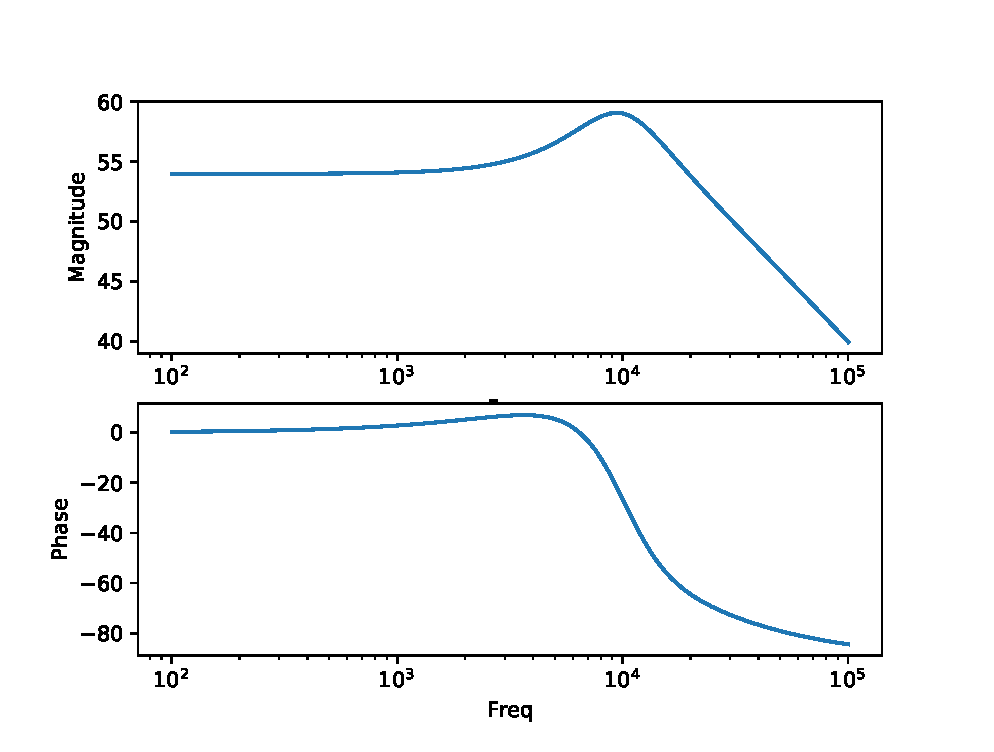
\includegraphics[width=\columnwidth]{./figs/ee18btech11038_bode.eps}
\caption{Bode Plot for $T(s)$}
\label{fig:ee18btech11038_bode}
\end{figure}

\item Simulate the circuit using spice.\\
\solution For simulation purpose, we will realise the closed loop amplifier as shown in Fig \ref{fig:ee18btech11038_sim} in spice.


\begin{figure}[!ht]
	\begin{center}
		
		\resizebox{\columnwidth}{!}{\begin{circuitikz}
\ctikzset{bipoles/length=1cm}
\draw (0,-0.5) node[]{} to [short](0,0.5) to [short](1,0) to [short](0,-0.5);

\draw (0.3, 0) node{$k$};
\draw (1,0) to [R=$R_2$](3,0) to [L=$L_2$](5,0) to [C=$C_2$](5,-3) node[ground]{};
\draw (5,0) to[short, -o] (6.5,0)node[right]{$v_{f}$};
\draw (6.5, -2)  to[vsource, l=$v_{i}$](6.5, -3) to node[ground]{}(6.5,-3);
\draw (6.5,-2) to[short, -o] (6.5,-1.5)node[right]{$v_{i}$};
\draw (6.5,0)node[below]{$-$};
\draw (6.5,-1.5)node[above]{$+$};
\draw (8, 0) to[cV, l =$10^3\times(v_{i}-v_{f})$](8,-2) to node[ground]{}(8,-2);
\draw (8,0) to [L = $L_{1}$ ](11.5,0) to [R=$R_{1}$](11.5,-2) to node[ground]{}(11.5,-2);
\draw (11.5,0) to[short, -o] (13,0)node[right]{$v_{o}$};
\draw (12.5, 0) to[short](12.5,-4) to[short](-1,-4) to[short](-1,0) to[short](0,0);
\end{circuitikz}}
	\end{center}
\caption{Circuit used for Simulation}
\label{fig:ee18btech11038_sim}
\end{figure}

\begin{align}
    R_{1}&= 1k\Omega \\
    L_{1}&= 100mH
\end{align}

\item Verify by results obtained using simulation\\
\solution Fig \ref{fig:ee18btech11038_freqres} shows the frequency response plot for the circuit in Fig \ref{fig:ee18btech11038_freqres} obtained using an A.C. sweep in spice.
You can find the netlist for the simulated circuit here:
\begin{lstlisting}
spice/ee18btech11038_opamp.cir
\end{lstlisting}
You can find the python script used to generate the output here:
\begin{lstlisting}
spice/ee18btech11038_opamp.py
\end{lstlisting}
\begin{figure}[!ht]
\centering
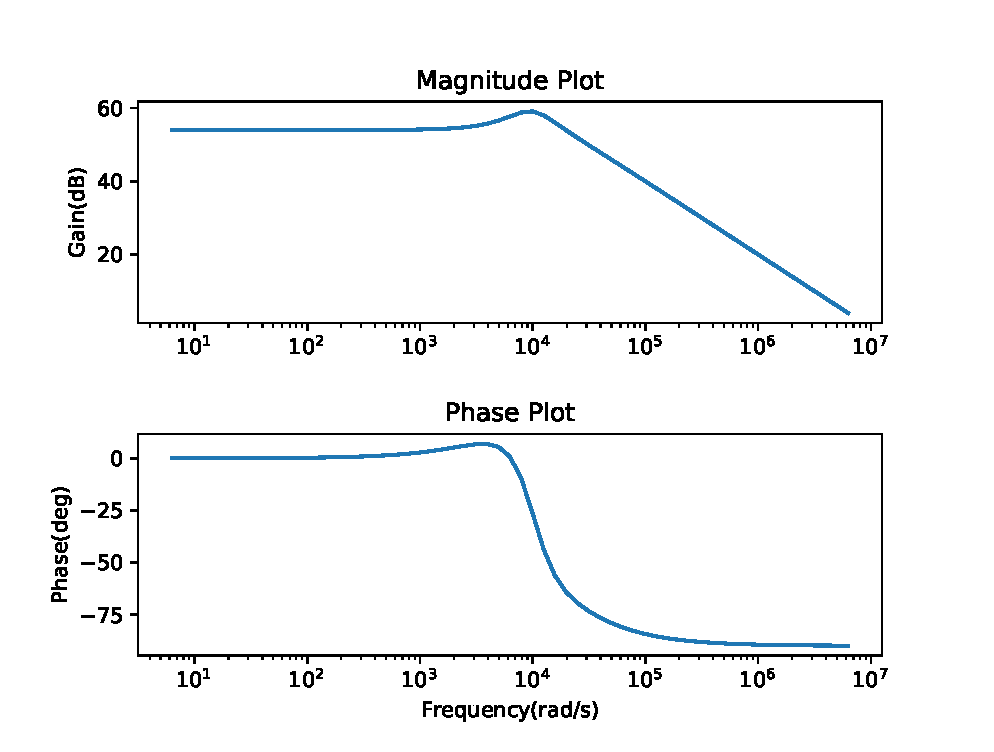
\includegraphics[width=\columnwidth]{./figs/ee18btech11038_freqres.eps}
\caption{Frequency Response from Simulation}
\label{fig:ee18btech11038_freqres}
\end{figure}

Clearly, the bode plot in Fig \ref{fig:ee18btech11038_bode} and plots in Fig \ref{fig:ee18btech11038_freqres} match. Hence verified.











\end{enumerate}


